% $Id$

The ESMF Time Manager utility includes software for time and time interval 
representation, as well as model time advancement. Since multi-component 
geophysical applications often require synchronization across 
the time management schemes of the individual components, the 
Time Manager's standard calendars and consistent time representation 
promote component interoperability.
\begin{center}  
\begin{tabular}{|p{6in}|}
\hline
\vspace{.01in}
{\bf Key Features} \\[.01in]
Drift-free timekeeping through an integer-based internal time 
representation.  Both integers and reals can be specified at the interface. \\
Support for many calendar kinds. \\
Support for both concurrent and sequential modes of component execution. \\[.03in] \hline
\end{tabular}
\end{center}

\subsection{Time Manager Classes}
There are four ESMF classes that represent time concepts:
\begin{itemize}
\item {\bf Calendar}  A Calendar can be used to keep track of the 
date as an ESMF Gridded Component advances in time. Standard calendars 
(such as Gregorian and 360-day) are supported. 
\item {\bf Time} A Time represents a time instant in a particular 
calendar, such as November 28, 1964, at 7:00pm EST in the Gregorian 
calendar.  The Time class can be used 
to represent the start and stop time of a time integration.
\item {\bf TimeInterval} TimeIntervals represent a period 
of time, such as 3 hours.  Time steps can be represented 
using TimeIntervals. 
\item {\bf Clock} Clocks collect the parameters and 
methods used for model time advancement into a convenient 
package.  A Clock can be queried for quantities such 
as current simulation time and time step.  Clock methods 
include incrementing the current time, and printing the its contents.
\end{itemize}

%\begin{center}
%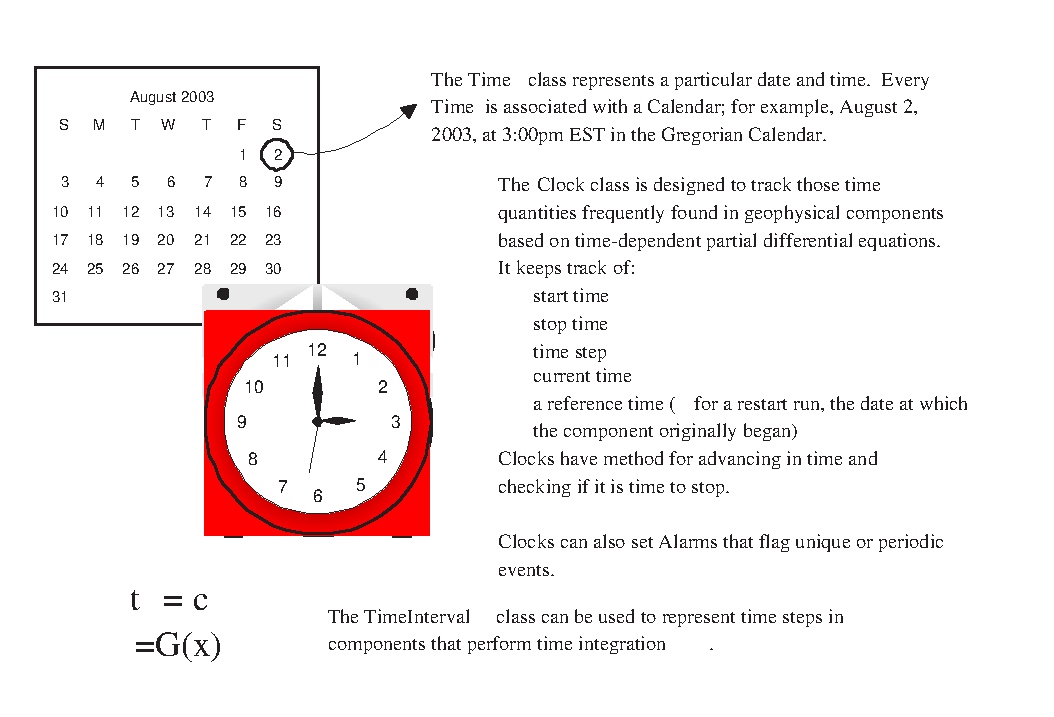
\includegraphics{TimeMgr_desc}
%\end{center}

%\newpage
%In the remainder of this section, we briefly summarize the 
%functionality that the Time Manager classes provide.  Detailed 
%descriptions and usage examples precede the API listing for each 
%class.

\subsection{Calendar}
The set of supported calendars includes:
\begin{description}
\item [Gregorian] The standard Gregorian calendar.
\item [no-leap] The Gregorian calendar with no leap years.
\item [Julian] The standard Julian date calendar.
\item [Julian Day] The standard Julian days calendar.
\item [Modified Julian Day] The Modified Julian days calendar.
\item [360-day] A 30-day-per-month, 12-month-per-year calendar.
\item [no calendar] Tracks only elapsed model time in hours, minutes, seconds.
\end{description}
See Section~\ref{sec:Calendar} for more details on supported standard 
calendars, and how to create a customized ESMF Calendar.

\subsection{Time Instants and TimeIntervals}
\label{subsec:Time Instants and TimeIntervals}
TimeIntervals and Time instants (simply called Times) are the computational 
building blocks of the Time Manager utility.  Times support different queries 
for values of individual Time components such as year and hour.
See Sections~\ref{sec:Time} and ~\ref{sec:TimeInterval}, respectively, 
for use of Times and TimeIntervals.

\subsection{Clocks}
It is useful to identify a higher-level concept to repeatedly step a Time 
forward by a TimeInterval.  We refer to this capability as a Clock, and 
include in its required features the ability to store the start and stop times 
of a model run, and to query the value of quantities such as the current time 
and the number of time steps taken.  Applications may contain 
temporary or multiple Clocks. Section~\ref{sec:Clock} describes the use of 
Clocks in detail.
